\chapter{Discussion} % Subjektiv discussion
This chapter will interpret the results outlined in the previous section and attempt to ground the solution in the previously presented theory.

\section{Overall Performance}
Overall, D1 was the best performing synthetic dataset. For the 10-shot task, it has an accuracy of 72.92, compared to 73.70 for the BL2 baseline. However, the disparity to the BL2 baseline increases as the number of few-shot samples decreases. For example, for the 5-shot task, this dataset have an accuracy of 67.83, compared to 72.88, a difference of roughly five percentage points. The best performing synthetic for the 5-shot class, dataset D5, was able to achieve 69.03 \% accuracy for the 5-shot tasks. In the 1-shot tasks, the best synthetic dataset D1 reached 46.41\% accuracy, roughly 16 percentage points the baseline of 62.94\%.

 %In comparison, on the 1-shot tasks, the best synthetic dataset D1 reached 46.41\% accuracy, roughly sixteen percentage points behind the BL2 baseline that reached 62.94\%.

\change{rewritten}
Based on these results, none of the synthetic datasets was able to force the models to learn domain agnostic features that could be used directly. However, as the number of examples in the few-shot tasks increases, the performance difference between the real-world dataset and the synthetic dataset is narrowed. This suggests that the synthetically trained networks can at least be quickly fine-tuned to the new real-world domain.

\section{Effect of Image Randomization}
Variation in lighting has a strong positive effect on the model's performance, similarly to what has been observed by \textcite{domainrand} and \textcite{goodsynthetic}. The difference between the best performing model trained with randomized light settings (using Dataset D1) and the model trained with a static light setting (using Dataset D2) is roughly eight percentage points for both 1-shot and 5-shot tasks (see Table \ref{accfiveone} and  \ref{accfivefive}). 

\textit{Crepuscular rays} (see Dataset D3) is the single lighting setting that has the most effect on performance. Disabling it results in roughly six to eight percentage points decrease in accuracy on all tasks. This result is not entirely surprising since randomizing the lighting into different colors fundamentally changes the nature of most scenes and introduces lots of visual variety.

Randomized \textit{weather} (see Dataset D4) had a lesser but noticeable effect. Disabling it results in a roughly six percentage point decrease in accuracy for the 10-shot class, two percentage points decrease in accuracy for the 5-shot task and a more than five percentage points decrease for the 1-shot task. It is not surprising that randomizing the weather affects accuracy. The weather itself is randomized across several variables and changes both brightness, image contrast, and introduces background noise with clouds, lightning, and rainbows.

On the other hand, randomizing \textit{time} (see Dataset D5) had a small effect possitive effect on the 10-shot task, a negative effect on the 5-shot task and a statistically insignificant effect in the 1-shot classification task. This result is unexpected since randomizing the time can often provide a high degree of variance to the images by re-positioning the primary light source. One possible reason why this could have a negative effect is that the shadows it generate made some of the vehicles too difficult to detect in the dataset. Another is that the test dataset does not have many images with lighting coming from the side. Therefore, making the network robust to this kind of dynamic lighting is a wasted effort.

Removing context (see Dataset D7) also hurts performance. Disabling it results in a reduction by one percentage point for the 1-shot classifier and more than two percentage points lower for the 5 and 10-shot classifiers. Similarly, randomizing textures (see Dataset D6) seems to have an overall negative effect. The result is a reduction by roughly two percentage points for the 1 and 10-shot classifier and 0.7 for the 5-shot classifier.

The standard deviation is high for all the tasks, but the real-world baseline (See Dataset BL2) does have a higher standard deviation than any of the synthetic datasets. The 5-shot classifiers also have a consistently lower standard deviation, which is to be expected since they are allowed to observe more data. The high standard deviation is a result of the test-set being small, but also a result of the military vehicle classification task in itself. Since some vehicles in the test data set are very similar and hard to distinguish, like different types of tanks or different types of airplanes, the difficulty of a sampled task can vary a lot depending on the visual similarity of the sampled classes.

In conclusion, randomizing light has an overall positive effect on performance for both tasks and can improve performance by several percentage points. Specifically, enabling crepuscular rays and randomizing weather seems to be the two most important factors. However, the exact randomization configuration that generates the best result, as well as the worst result, differs slightly between the 1-shot and 5-shot tasks.

\section{Realism vs. Visual Variety}
A common question when generating synthetic data is how visually similar it must be in order to be useful for training. Out of the seven generated datasets, D3 is the one which is most visually similar to the real-world test data. This dataset has realistic vehicle positions, lighting without any god rays, no randomized vehicle textures, and variations in both lighting direction and weather. As can be seen in Tables \ref{accfiveone} and  \ref{accfivefive}, this dataset is outperformed by all datasets for the 1 and 10-shot tasks and all except D2 for 5-shot tasks. These results suggest that aiming for visual realism, while reducing the visual variety, can result in lower accuracy. This result, that variation can be more important than realism, is similar to what has been discovered in much previous research~\cite{goodsynthetic, domainrand, domainrandcars}.

It would be convenient if synthetic data did not have to be realistic at all since it would make the data generation process easier. However, merely adding more visual variety does not correlate with improved performance either. This phenomenon is most evident with dataset D5, which is less varied than D1, while still being able to outperform it on the 5-shot tasks. Similarly, positioning the models unrealistically, and randomizing textures also harmed performance, as seen with datasets D7 and D6 on both tasks.

These results raise the question about what aspects of synthetic data should be randomized in order to improve performance. \textcite{structureddomainrandomization} argues in their paper that using knowledge about the application domain, which they call context, can be more beneficial than simply introducing more visual variety in the synthetic data. For example, they generated synthetic images for the task of car detection. The images that they used as test data were all taken in in traffic with a camera mounted to a car. Therefore, the synthetic images were generated to always be on a road, and they always positioned the simulation camera to be in a similar position as the test images. However, aspects that changed in the dataset, such as lighting, roads, background, and weather, were heavily randomized in the dataset. 

The test-set used in this thesis do not come from one source, and therefore, it is difficult to make these kinds of assumptions, both about context or about the camera. One thing which is known, however, is that the vehicles are always positioned realistically, which could explain why simply positioning the vehicles randomly, like in dataset D7, harms performance. Similarly, the vehicles in each class in the test-set are generally of the same color or similar colors, which could explain why randomizing vehicle textures did not improve performance.

In conclusion, our hypothesis is that good synthetic data should be randomized along dimensions that make the network robust to the domain shift between synthetic and real data. For vehicle classification, these dimensions seem to be mostly related to the light setting. The images should also be randomized along the dimensions which are varied in the test domain, in order for the model to properly learn the tasks. However, randomizing along the dimensions which are not varied in the test data, nor contribute to the domain shift, such as vehicle positions in our experiments, can have a negative effect, since it needlessly raises the difficulty of the training task.

\section{The Effect of Task Difficulty}
By using synthetic data, there is an opportunity to investigate how changing certain aspects of the data can affect the meta-learning process. An interesting phenomenon that can be seen in the training plots is how the training accuracy plummets during earlier update steps for models trained on specific datasets. In the 5-way classification task (see Figures \ref{subplot:fivefiveone}--\ref{subplot:fivefivefive}) it is the more randomized datasets (D1, D5, D7, D6) that drops in accuracy after the first and second update step. Similarly, for the 1-shot task (see Figures \ref{subplot:fiveoneone}--\ref{subplot:fiveonefive}) it is the least randomized datasets (D2, D4, D3) who drops in accuracy during the two first updates. \textcite{reptile} hypothesize in their paper that their Reptile algorithm, converges towards a parameter setting that is the closest, in terms of Euclidean distance, to the manifold of optimal solutions for each of the training tasks. Assuming that a similar type convergence occurs in MAML, the drop in accuracy in the early steps could be due to a high visual variety in the generated task, which results in a more considerable on-average distance between the task manifolds. As a result, the network would need more fine-tuning steps in order to reach the manifolds, which would explain why the accuracy plummets in the earlier steps.

One problem with this theory is that the drop in validation accuracy happens to different datasets between the 5-shot and the 1-shot classifiers. If the theory held the accuracy for the D2 dataset would not decrease, but rather all the other. Therefore, further research into how task-difficulty, stochastic gradient descent, and MAML all affect the ability of the network to generalization is needed before a solid conclusion can be drawn.

\section{Are We Actually Learning?}
Even though the test-accuracy of a model is a good indication of how a model will perform in the real world, it does not show what the model has learned. It can, therefore, be a good idea to ascertain that the model is learning what one intends for it to learn. Ensuring that a model learns properly is especially crucial when data is limited, and when a model is applied to a new target domain, which is the case for synthetic meta-learning.

To accomplish this, one can use one of the many recently developed \gls{XAI} methods to visualize what parts of the image that influence the network's decision making. Figure \ref{grad-cam-5-5} shows a few examples of Grad-Cam~\cite{gradcam} visualization. The images and heatmaps showcase how the 5-way 5-shot model, trained with the D1 dataset, changes what pixels influence its decision after each update. These example images all consist of previously unseen validation data that was not used by the network during these five update steps. The five training samples are shown in Figure \ref{grad-cam-training-5-5}.

\begin{figure}[H]
\centering
\subcaptionbox{0 steps}
  {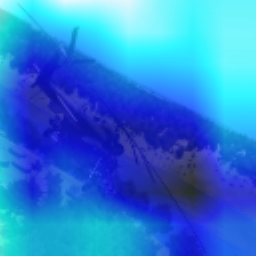
\includegraphics[height=2.4cm, width=2.4cm]{images/vbs3/gradcam/5-5/1/Heat_map_of_iterations_0.png}}
\subcaptionbox{1 step}
  {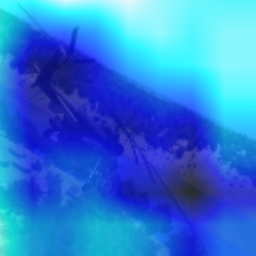
\includegraphics[height=2.4cm, width=2.4cm]{images/vbs3/gradcam/5-5/1/Heat_map_of_iterations_1.png}}
\subcaptionbox{3 steps}
  {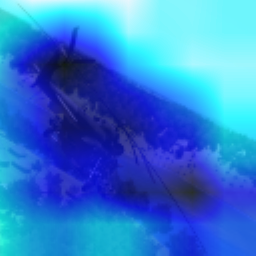
\includegraphics[height=2.4cm, width=2.4cm]{images/vbs3/gradcam/5-5/1/Heat_map_of_iterations_3.png}}
\subcaptionbox{5 steps}%
  {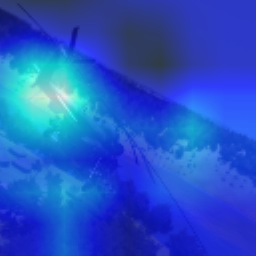
\includegraphics[height=2.4cm, width=2.4cm]{images/vbs3/gradcam/5-5/1/Heat_map_of_iterations_5.png}}
\subcaptionbox{Image}
  {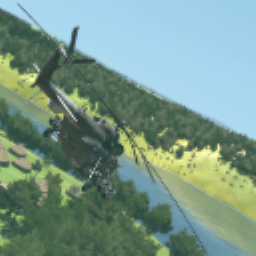
\includegraphics[height=2.4cm, width=2.4cm]{images/vbs3/gradcam/5-5/1/Test_Images.png}}


\subcaptionbox{0 steps}
  {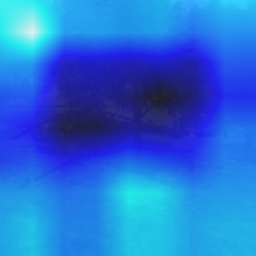
\includegraphics[height=2.4cm, width=2.4cm]{images/vbs3/gradcam/5-5/2/Heat_map_of_iterations_0.png}}
\subcaptionbox{1 step}
  {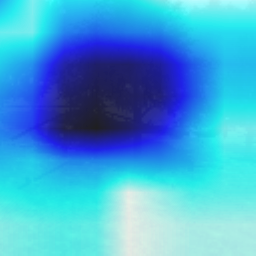
\includegraphics[height=2.4cm, width=2.4cm]{images/vbs3/gradcam/5-5/2/Heat_map_of_iterations_1.png}}
\subcaptionbox{3 steps}
  {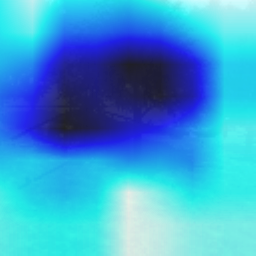
\includegraphics[height=2.4cm, width=2.4cm]{images/vbs3/gradcam/5-5/2/Heat_map_of_iterations_3.png}}
\subcaptionbox{5 steps}%
  {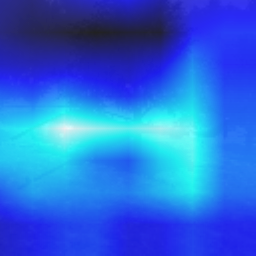
\includegraphics[height=2.4cm, width=2.4cm]{images/vbs3/gradcam/5-5/2/Heat_map_of_iterations_5.png}}
\subcaptionbox{Image}
  {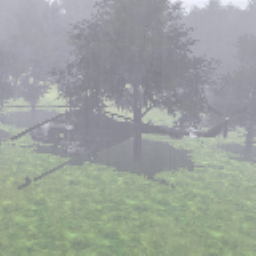
\includegraphics[height=2.4cm, width=2.4cm]{images/vbs3/gradcam/5-5/2/Test_Images.png}}
  
\subcaptionbox{0 steps}
  {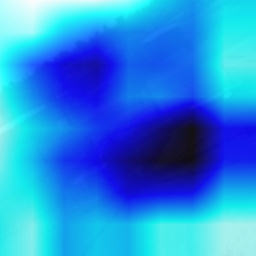
\includegraphics[height=2.4cm, width=2.4cm]{images/vbs3/gradcam/5-5/3/Heat_map_of_iterations_0.png}}
\subcaptionbox{1 step}
  {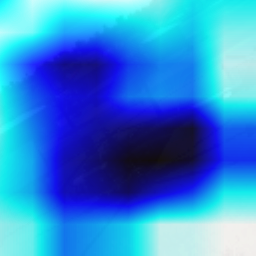
\includegraphics[height=2.4cm, width=2.4cm]{images/vbs3/gradcam/5-5/3/Heat_map_of_iterations_1.png}}
\subcaptionbox{3 steps}
  {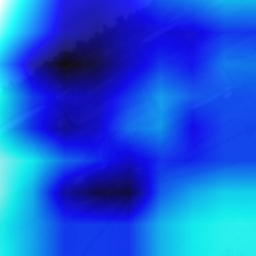
\includegraphics[height=2.4cm, width=2.4cm]{images/vbs3/gradcam/5-5/3/Heat_map_of_iterations_3.png}}
\subcaptionbox{5 steps}%
  {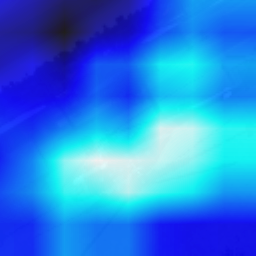
\includegraphics[height=2.4cm, width=2.4cm]{images/vbs3/gradcam/5-5/3/Heat_map_of_iterations_5.png}}
\subcaptionbox{Image}
  {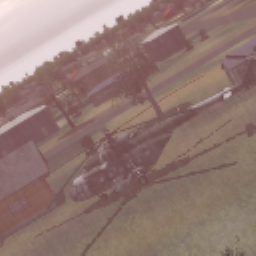
\includegraphics[height=2.4cm, width=2.4cm]{images/vbs3/gradcam/5-5/3/Test_Images.png}}
  
\caption{Network attention on unseen validation samples during training for \textbf{5-way 1-shot} tasks using D1. Lighter color indicates the pixel have more influence on the final prediction}
\label{grad-cam-5-5}
\end{figure}

\begin{figure}[H]
\centering
\subcaptionbox{}
  {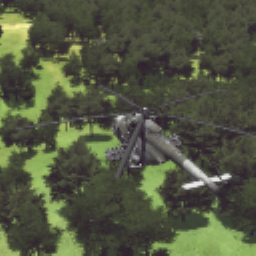
\includegraphics[height=2.4cm, width=2.4cm]{images/vbs3/gradcam/5-5/train/Test_Images-1.png}}
\subcaptionbox{}
  {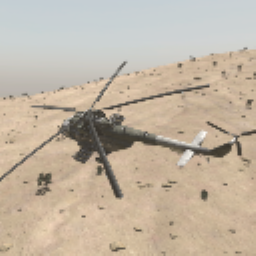
\includegraphics[height=2.4cm, width=2.4cm]{images/vbs3/gradcam/5-5/train/Test_Images-2.png}}
\subcaptionbox{}
  {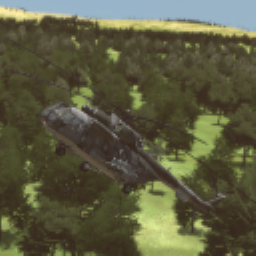
\includegraphics[height=2.4cm, width=2.4cm]{images/vbs3/gradcam/5-5/train/Test_Images-3.png}}
\subcaptionbox{}
  {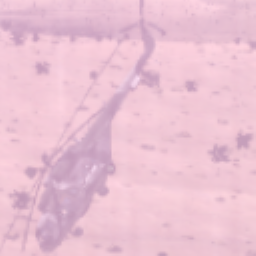
\includegraphics[height=2.4cm, width=2.4cm]{images/vbs3/gradcam/5-5/train/Test_Images-4.png}}
\subcaptionbox{}
  {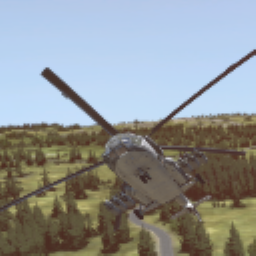
\includegraphics[height=2.4cm, width=2.4cm]{images/vbs3/gradcam/5-5/train/Test_Images-5.png}}
\caption{Training data for 5-way 5-shot}
\label{grad-cam-training-5-5}  
\end{figure}

In Figure \ref{grad-cam-5-5}, the attention displayed shows that the helicopter, or parts of it, are the most influential parts of the validation images. The networks ability to consistently locate the helicopter suggests that the network has learned to find the object in the image, regardless of image filter, rotation, and obfuscation. This is a good indicator that it has learned the given task successfully.

\begin{figure}[H]
\centering
\subcaptionbox{0 steps}
  {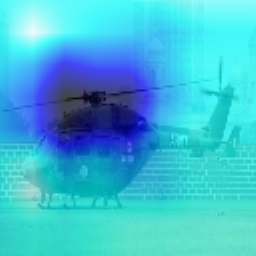
\includegraphics[height=2.4cm, width=2.4cm]{images/real-images/gradcam/5-5/1/Heat_map_of_iterations_0.png}}
\subcaptionbox{1 step}
  {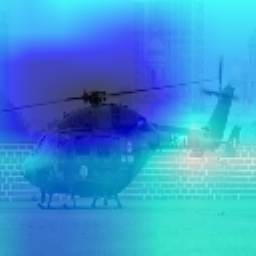
\includegraphics[height=2.4cm, width=2.4cm]{images/real-images/gradcam/5-5/1/Heat_map_of_iterations_1.png}}
\subcaptionbox{3 steps}
  {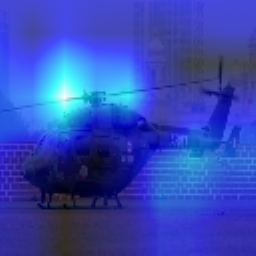
\includegraphics[height=2.4cm, width=2.4cm]{images/real-images/gradcam/5-5/1/Heat_map_of_iterations_3.png}}
\subcaptionbox{5 steps}%
  {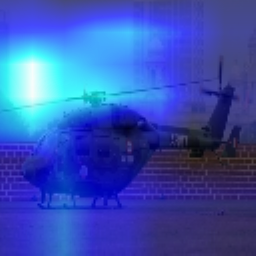
\includegraphics[height=2.4cm, width=2.4cm]{images/real-images/gradcam/5-5/1/Heat_map_of_iterations_5.png}}
\subcaptionbox{Image}
  {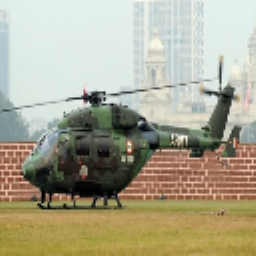
\includegraphics[height=2.4cm, width=2.4cm]{images/real-images/gradcam/5-5/1/Test_Images.png}}

\subcaptionbox{0 steps}
  {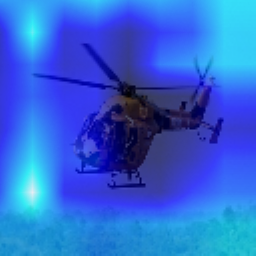
\includegraphics[height=2.4cm, width=2.4cm]{images/real-images/gradcam/5-5/2/Heat_map_of_iterations_0.png}}
\subcaptionbox{1 step}
  {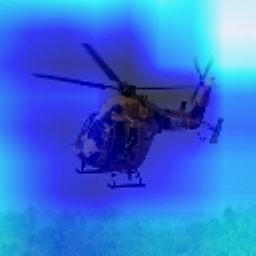
\includegraphics[height=2.4cm, width=2.4cm]{images/real-images/gradcam/5-5/2/Heat_map_of_iterations_1.png}}
\subcaptionbox{3 steps}
  {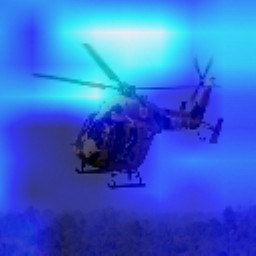
\includegraphics[height=2.4cm, width=2.4cm]{images/real-images/gradcam/5-5/2/Heat_map_of_iterations_3.png}}
\subcaptionbox{5 steps}%
  {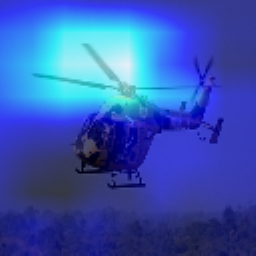
\includegraphics[height=2.4cm, width=2.4cm]{images/real-images/gradcam/5-5/2/Heat_map_of_iterations_5.png}}
\subcaptionbox{Image}
  {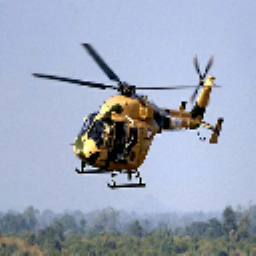
\includegraphics[height=2.4cm, width=2.4cm]{images/real-images/gradcam/5-5/2/Test_Images.png}}
  
\subcaptionbox{0 steps}
  {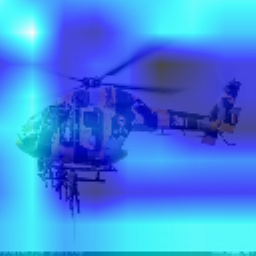
\includegraphics[height=2.4cm, width=2.4cm]{images/real-images/gradcam/5-5/3/Heat_map_of_iterations_0.png}}
\subcaptionbox{1 step}
  {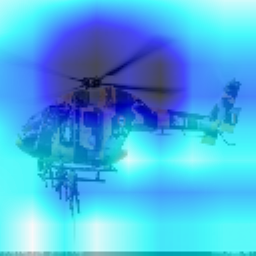
\includegraphics[height=2.4cm, width=2.4cm]{images/real-images/gradcam/5-5/3/Heat_map_of_iterations_1.png}}
\subcaptionbox{3 steps}
  {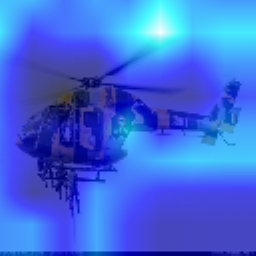
\includegraphics[height=2.4cm, width=2.4cm]{images/real-images/gradcam/5-5/3/Heat_map_of_iterations_3.png}}
\subcaptionbox{5 steps}%
  {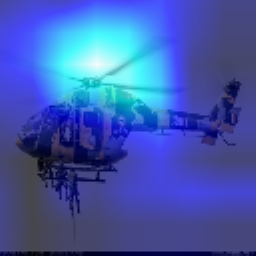
\includegraphics[height=2.4cm, width=2.4cm]{images/real-images/gradcam/5-5/3/Heat_map_of_iterations_5.png}}
\subcaptionbox{Image}
  {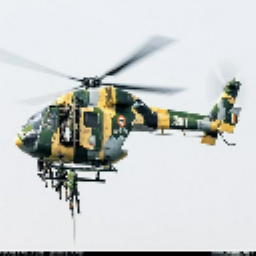
\includegraphics[height=2.4cm, width=2.4cm]{images/real-images/gradcam/5-5/3/Test_Images.png}}
  
\caption{Network attention on unseen real-world test samples for \textbf{5-way 5-shot} tasks. Lighter color indicates the pixel have more influence on the final prediction}
\label{grad-cam-real-5-5}
\end{figure}

The same visualization technique can also be applied to the real test data during the meta-test phase, in order to ensure that this ability to learn is carried over during the domain transition from synthetic to real data. Some examples can be seen in Figure \ref{grad-cam-real-5-5}. These example images suggest that the model can locate at least a part of the object of interest in all images. However, in this example, it is only able to find the rotor of the helicopter, while the body is seemingly ignored. The focus on the rotor is most likely a result of this model having been trained on vehicle models with more consistent coloring, while the real-world vehicles in the test-set can have varied colors.


In contrast, for the 5-way 1-shot classification task, the model appears less reliable in finding the object of interest. Both for the training data (see Figure \ref{grad-cam-5-1} and Figure \ref{grad-cam-training}) and the real-world test data (see Figure \ref{grad-cam-real-5-1}). 

\begin{figure}[H]
\centering
\subcaptionbox{0 steps}
  {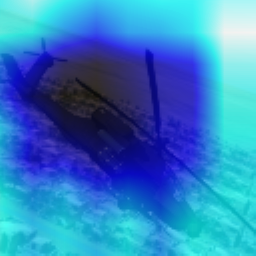
\includegraphics[height=2.4cm, width=2.4cm]{images/vbs3/gradcam/5-1/1/Heat_map_of_iterations_0.png}}
\subcaptionbox{1 step}
  {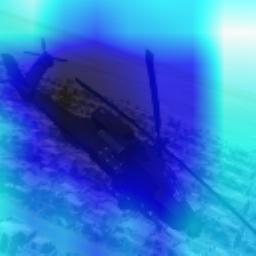
\includegraphics[height=2.4cm, width=2.4cm]{images/vbs3/gradcam/5-1/1/Heat_map_of_iterations_1.png}}
\subcaptionbox{3 steps}
  {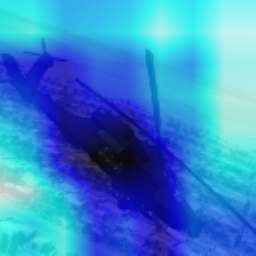
\includegraphics[height=2.4cm, width=2.4cm]{images/vbs3/gradcam/5-1/1/Heat_map_of_iterations_3.png}}
\subcaptionbox{5 steps}%
  {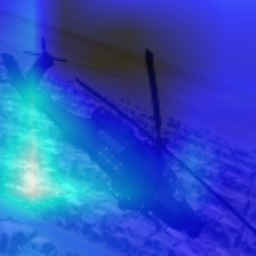
\includegraphics[height=2.4cm, width=2.4cm]{images/vbs3/gradcam/5-1/1/Heat_map_of_iterations_5.png}}
\subcaptionbox{Image}
  {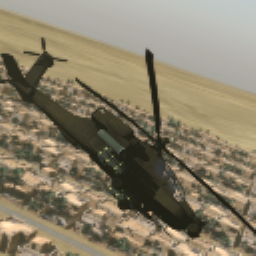
\includegraphics[height=2.4cm, width=2.4cm]{images/vbs3/gradcam/5-1/1/Test_Images.png}}


\subcaptionbox{0 steps}
  {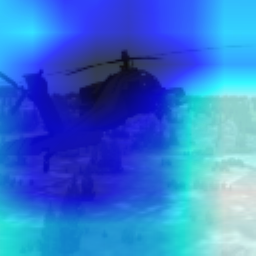
\includegraphics[height=2.4cm, width=2.4cm]{images/vbs3/gradcam/5-1/2/Heat_map_of_iterations_0.png}}
\subcaptionbox{1 step}
  {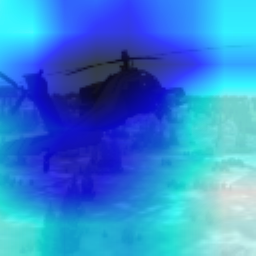
\includegraphics[height=2.4cm, width=2.4cm]{images/vbs3/gradcam/5-1/2/Heat_map_of_iterations_1.png}}
\subcaptionbox{3 steps}
  {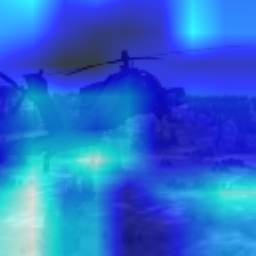
\includegraphics[height=2.4cm, width=2.4cm]{images/vbs3/gradcam/5-1/2/Heat_map_of_iterations_3.png}}
\subcaptionbox{5 steps}%
  {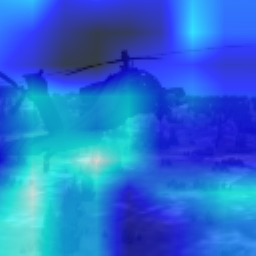
\includegraphics[height=2.4cm, width=2.4cm]{images/vbs3/gradcam/5-1/2/Heat_map_of_iterations_5.png}}
\subcaptionbox{Image}
  {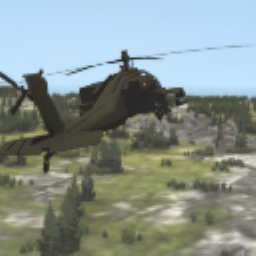
\includegraphics[height=2.4cm, width=2.4cm]{images/vbs3/gradcam/5-1/2/Test_Images.png}}
  
\subcaptionbox{0 steps}
  {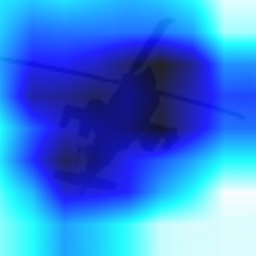
\includegraphics[height=2.4cm, width=2.4cm]{images/vbs3/gradcam/5-1/3/Heat_map_of_iterations_0.png}}
\subcaptionbox{1 step}
  {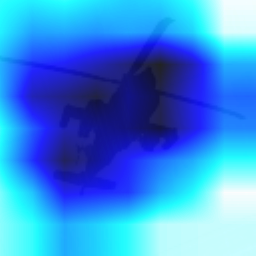
\includegraphics[height=2.4cm, width=2.4cm]{images/vbs3/gradcam/5-1/3/Heat_map_of_iterations_1.png}}
\subcaptionbox{3 steps}
  {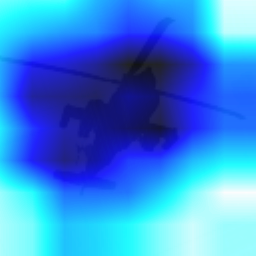
\includegraphics[height=2.4cm, width=2.4cm]{images/vbs3/gradcam/5-1/3/Heat_map_of_iterations_3.png}}
\subcaptionbox{5 steps}%
  {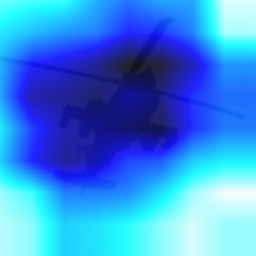
\includegraphics[height=2.4cm, width=2.4cm]{images/vbs3/gradcam/5-1/3/Heat_map_of_iterations_5.png}}
\subcaptionbox{Image}
  {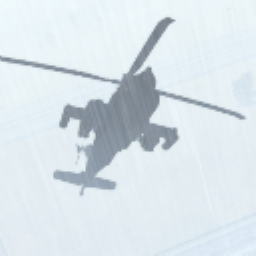
\includegraphics[height=2.4cm, width=2.4cm]{images/vbs3/gradcam/5-1/3/Test_Images.png}}
  
\caption{GradCam-visualization on unseen validation samples during training for \textbf{5-way 1-shot} tasks using D1. Lighter color indicates the pixel have more influence on the final prediction}
\label{grad-cam-5-1}
\end{figure}

\begin{figure}[H]
\centering
\subcaptionbox{}
  {\includegraphics[height=2.4cm, width=2.4cm]{images/vbs3/gradcam/5-1/train/Test_Images.png}}
\label{grad-cam-training}  
\caption{Training data for 5-way 1-shot}
\end{figure}


\begin{figure}[H]
\centering
\subcaptionbox{0 steps}
  {\includegraphics[height=2.4cm, width=2.4cm]{images/real-images/gradcam/5-1/1/Heat_map_of_iterations_0.png}}
\subcaptionbox{1 step}
  {\includegraphics[height=2.4cm, width=2.4cm]{images/real-images/gradcam/5-1/1/Heat_map_of_iterations_1.png}}
\subcaptionbox{3 steps}
  {\includegraphics[height=2.4cm, width=2.4cm]{images/real-images/gradcam/5-1/1/Heat_map_of_iterations_3.png}}
\subcaptionbox{5 steps}%
  {\includegraphics[height=2.4cm, width=2.4cm]{images/real-images/gradcam/5-1/1/Heat_map_of_iterations_5.png}}
\subcaptionbox{Image}
  {\includegraphics[height=2.4cm, width=2.4cm]{images/real-images/gradcam/5-1/1/Test_Images.png}}


\subcaptionbox{0 steps}
  {\includegraphics[height=2.4cm, width=2.4cm]{images/real-images/gradcam/5-1/2/Heat_map_of_iterations_0.png}}
\subcaptionbox{1 step}
  {\includegraphics[height=2.4cm, width=2.4cm]{images/real-images/gradcam/5-1/2/Heat_map_of_iterations_1.png}}
\subcaptionbox{3 steps}
  {\includegraphics[height=2.4cm, width=2.4cm]{images/real-images/gradcam/5-1/2/Heat_map_of_iterations_3.png}}
\subcaptionbox{5 steps}%
  {\includegraphics[height=2.4cm, width=2.4cm]{images/real-images/gradcam/5-1/2/Heat_map_of_iterations_5.png}}
\subcaptionbox{Image}
  {\includegraphics[height=2.4cm, width=2.4cm]{images/real-images/gradcam/5-1/2/Test_Images.png}}
  
\subcaptionbox{0 steps}
  {\includegraphics[height=2.4cm, width=2.4cm]{images/real-images/gradcam/5-1/3/Heat_map_of_iterations_0.png}}
\subcaptionbox{1 step}
  {\includegraphics[height=2.4cm, width=2.4cm]{images/real-images/gradcam/5-1/3/Heat_map_of_iterations_1.png}}
\subcaptionbox{3 steps}
  {\includegraphics[height=2.4cm, width=2.4cm]{images/real-images/gradcam/5-1/3/Heat_map_of_iterations_3.png}}
\subcaptionbox{5 steps}%
  {\includegraphics[height=2.4cm, width=2.4cm]{images/real-images/gradcam/5-1/3/Heat_map_of_iterations_5.png}}
\subcaptionbox{Image}
  {\includegraphics[height=2.4cm, width=2.4cm]{images/real-images/gradcam/5-1/3/Test_Images.png}}
  
  \caption{GradCam-visualization on unseen real-world test samples for \textbf{5-way 1-shot tasks}. Lighter color indicates the pixel have more influence on the final prediction}
  \label{grad-cam-real-5-1}
\end{figure}

\change{New section}
\section{Validity of the baselines}
This section will cover some of the issues with the baselines used in this thesis, to indicate what could be amended in future research.

For the first baseline, no explicit hyperparameter search was done. Instead, it used the same parameters as all the other models. This was a result of time constraints when performing the experiments. It is therefore possible that this baseline underperforms compared to its best possible instance, since there is no guarantee that these parameter settings are the best possible ones.

For the second baseline there is an issue with the number of samples. The training dataset consist of 9954 samples, 62 classes with 80 to 300 samples. As a comparison, the miniImageNet dataset~\cite{matching} consists of 80 training classes with 600 images each, a total of 48,000 test images. As a result, this thesis' baseline is allowed to observe roughly 4.8 times less data than a model trained on miniImageNet. Also, the models trained with synthetic data have access to roughly 106,000 synthetic images. As a result, this baseline might not seem like an entirely fair comparison. However, this was the number of real-world images which could be collected by a single-man team in a couple of days. This highlights one of the problems with the hand-labeled approach since this dataset took several days to assemble, clean, and prepare. In comparison, creating a new dataset using the simulator takes roughly 6 hours.

\section{Ethics and Sustainability}
From an ethical point of view, meta-learning, and in particular synthetic meta-learning have the potential of democratizing deep learning technology. Since deep learning requires large amounts of data, the state-of-the-art in machine learning is mostly done by large organizations that have access to ever-increasing amounts of data. If training efficient deep learning models did not require any actual data, but rather easily generated synthetic data and a handful of real-world examples, the number of people who could use and benefit from deep learning would increase significantly. 

Meta-Learning can also offer increased sustainability. Training contemporary state-of-the-art neural networks is a highly energy consuming task. Deep neural networks are often trained for days or even weeks on energy consuming hardware. Meta-learning offers a more energy-conserving approach to training. With meta-training, a very general pre-trained model can be trained in a couple of hours. This model can then later be trained for a broad range of different tasks in only a handful of update steps. If this technique could be perfected enough to rival state-of-the-art approaches, it would, therefore, remove the need for the long, energy consuming training process and thus decrease overall energy consumption.
